\documentclass{article}
\usepackage[polish]{babel}
\usepackage[T1]{fontenc}
\usepackage[a4paper, margin=1in]{geometry}

\usepackage{tikz}
\usetikzlibrary{quotes,angles,calc,patterns}
\usetikzlibrary{shapes.geometric}
\usepackage{float}
\usepackage{booktabs}
\usepackage{nicefrac}
\usepackage{amsmath}
\usepackage{pgfplots}
\usepackage{hyperref}

\title{FairPair -- Dokumentacja}
\author{REDACTED}

\begin{document}
\maketitle

\section{Problemy do rozwiązania przed rozpoczęciem realizacji}

Zanim nasz projekt zostanie wcielony w życie, musimy zastanowić się, jak
podzielić się zadaniami.  Będzie to ważny czynnik, umożliwiający sprawną
współpracę, ponieważ czeka nas kilka zadań, które mogą zająć nam więcej czasu.
Przykładem takich zadań są napisanie kodu do komunikacji z serwerem lub
front end. Żaden z członków zespołu nie ma zbyt dużego doświadczenia w tych
dziedzinach, więc będziemy musieli założyć, że zajmie nam to dużo czasu.

Kolejnym problemem jest dobór języków/środowisk/narzędzi, na których będziemy
opierać nasz program. Ze względu na szeroki zakres funkcjonalności, będziemy
musieli skorzystać z wielu technologii.  Przeszkodą może tu być komunikacja
pomiędzy poszczególnymi segmentami, dlatego też przed rozpoczęciem implementacji
musimy dokładnie przemyśleć, z czego chcemy skorzystać. Skłaniamy się
najbardziej ku popularnym rozwiązaniom, ponieważ mają one często gotowe
wtyczki/frameworki, umożliwiające komunikację z innymi technologiami oraz mają
ogromne wsparcie.

\section{Opis ograniczeń}
Najważniejszym ograniczeniem, które zostało narzucone, jest
ograniczenie czasowe. Musimy dostarczać konkretne fragmenty programu w
wyznaczonym czasie, więc nie możemy sobie pozwolić na opóźnienia na
żadnym etapie projektu (na szczęście mamy przygotowane plany awaryjne,
które mogą pomóc nam zmieścić się w ramach czasowych).

Czynnikiem bezpośrednio ograniczającym działanie aplikacji jest fakt, że
serwer nie będzie działał cały czas -- będzie uruchamiany tylko na czas
testów. Spowoduje to, że eksperci nie będą mieć dostępu do wyników
historycznych rankingów. Jest to pewna niedogodność, którą musimy mieć
na uwadze, jednak nie powinna ona przeszkodzić w przeprowadzeniu
finalnych testów podczas laboratoriów.

\section{Metodologia projektowa}
Mając na uwadze strukturę projektu oraz ograniczenia (głównie
czasowe) przyjmiemy metodologię waterfall. Dzięki dokładnym wytycznym,
dotyczącym poszczególnych aspektów projektu, możemy już na początku
opracować dokładny plan działania. Liczymy się z tym, że funkcjonalną
wersję aplikacji dostarczymy dość późno, jednak nie widzimy innej opcji,
więc będziemy się trzymać tej metodologii.

\section{Ogólny opis założeń architektonicznych}

\subsection{Plan główny}

Aplikacja będzie się składała z kilku komponentów (baza danych,
aplikacja webowa eksperta, aplikacja webowa admina, program do
generowania wyników rankingu), które będą wymagały różnych narzędzi
programistycznych. Jednym z nich jest FastAPI -- framework, umożliwiający
tworzenie interfejsów RESTful API w języku Python. Do implementacji bazy
danych użyjemy SQLite. Żeby ograniczyć liczbę
języków programowania, program do obliczania wyników rankingu również
zostanie zaimplementowany w języku Python (z użyciem biblioteki Numpy,
dla przyspieszenia obliczeń). Front-end aplikacji webowych zostanie
zaimplementowany w języku Rust używając technologii WebAssembly.

Elementem projektu, który nie został z góry narzucony, jest sposób
udostępniania rankingów ekspertom. Naszym pomysłem na rozwiązanie tej
kwestii jest wysyłanie tokenów- ekspert, który otrzyma dany token,
będzie mógł wziąć udział w rankingu i zobaczyć jego wyniki. Token będzie
mógł być udostępniany np. mailowo.

\subsection{Plan awaryjny}

Jeśli implementacja połączenia z bazą danych z pomocą frameworku FastAPI nie
powiedzie się, użyjemy frameworku Django, który
jest najpopularniejszym rozwiązaniem do pracy z bazami danych w języku
Python.

W przypadku, kiedy nie uda się zaimplementować systemu wysyłania tokenów
do ekspertów, planujemy dać ekspertom możliwość uwierzytelniania się
mailem. Ekspert po zalogowaniu się będzie widział listę udostępnionych
mu rankingów, w których może wziąć udział.

\section{Szczegółowy opis architektury}

\textbf{Link do repozytorium z kodem: }
\url{https://github.com/funsafe-math/ranking\_project}

\subsection{BAZA DANYCH}

Diagram bazy danych został przedstawiony na rysunku \ref{fig:database}. Dzięki
zaimplementowaniu jej w ten sposób, będziemy mogli przechowywać dane
historycznych rankingów. Poszczególne tabele będą zaimplementowane w
języku Python z pomocą biblioteki Pydantic.

\begin{figure}[H]
  \centering
  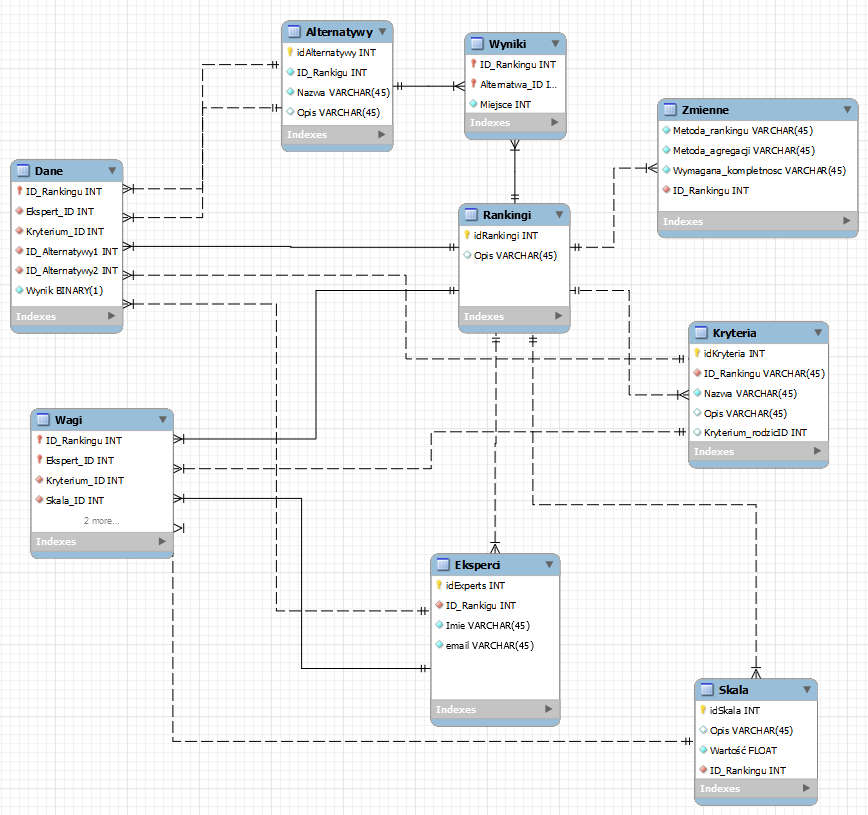
\includegraphics[width=0.9\textwidth]{Pictures/10000201000003640000032FB1B8D35E8021B7E0.png}

  \caption{\label{fig:database}Schemat bazy danych}
\end{figure}


\subsection{SERWER (ADMIN)}

Admin będzie zarządzał serwerem, w którego kodzie będzie
zaimplementowana baza danych (razem z funkcjami do jej obsługi). Oznacza
to, że aplikacja eksperta oraz program do obliczania rankingów będą
musiały komunikować się z adminem, żeby uzyskać informacje o 
rankingach. Pomimo tego, że logika serwera i baza danych będą
współdzielić część plików kodu, będą one miały osobne funkcje i będą
dziedziczyły po innych klasach, przez co ogólny schemat architektoniczny
(rysunek \ref{fig:architecture}) zostanie zachowany.

\begin{figure}[H]
  \centering
  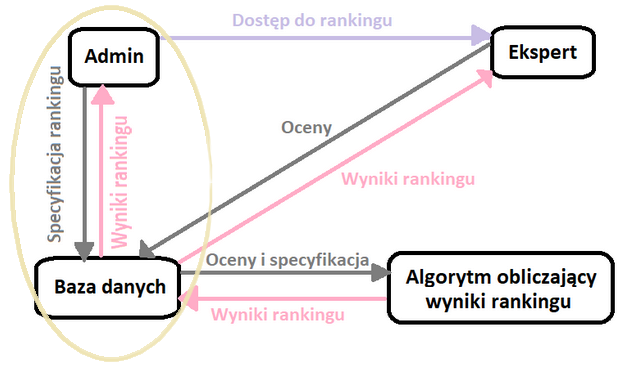
\includegraphics[width=0.7\textwidth]{Pictures/10000201000002710000017D1497C621F04447B6.png}

  \caption{\label{fig:architecture}Ogólny zarys architektury (baza danych i admin działają
razem)}
\end{figure}

\subsection{KLIENT (EKSPERT)}

Aplikacja klienta będzie bazowała na podobnych założeniach jak aplikacja
admina- jej front-end i back-end zostaną zaimplementowane z użyciem tych
samych języków i bibliotek. Umożliwi to bezproblemową komunikację między
adminem a ekspertem.

\subsection{FRONT-END}

Docelowo nasz program ma mieć możliwość obsługi przez klienta i admina z
telefonu, dlatego front-end aplikacji webowych zaimplementujemy w języku
Rust. Projekt frontendu aplikacji webowych (dwa widoki eksperta i jeden
admina) jest widoczny na rysunku \ref{fig:gui}. W finalnej wersji admin
będzie miał jeszcze odpowiedni widok do udostępniania rankingu
ekspertom, jednak ten widok będzie musiał być dostosowany do strategii
udostępniania, którą finalnie zaimplementujemy.

\begin{figure}[H]
  \centering
  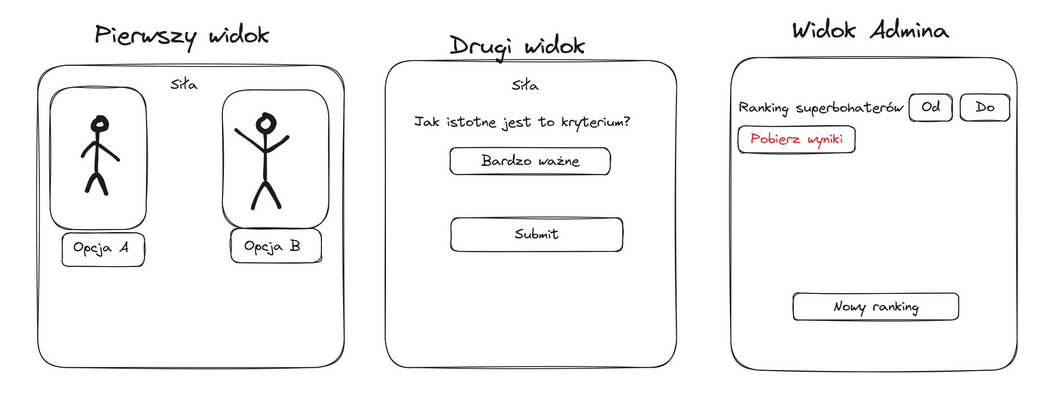
\includegraphics[width=0.9\textwidth]{Pictures/10000201000004180000018B4A3831CB6AABDC44.png}

  \caption{\label{fig:gui}Projekt dwóch widoków eksperta i jednego widoku admina}
\end{figure}

\section{Słownik pojęć}

\begin{itemize}
  \item Alternatywa: Możliwość, wybór spośród różnych opcji

  \item Kryterium: Cecha, według której dokonywane jest porównanie alternatyw

  \item Ekspert: Osoba posiadająca wiedzę i doświadczenie w danej dziedzinie,
oceniająca ranking

  \item Ocena: Opinia eksperta na temat porównania alternatyw w kontekście
danego kryterium

  \item Ranking: Zbiór alternatyw ocenianych w określonym kontekście
\end{itemize}

\end{document}